\chapter{Lösungsansatz}
\label{chap:Textsatz}
Mithilfe der Informationen aus der Problemfeldanalyse wurde eine mögliche Lösung für das Problem entwickelt. 
Im Rahmen des Praxisprojektes sollte so ein Lernsystem für Git und GitHub entwickelt werden, in dem Studierende 
sich selbst Wissen aneignen können, und dieses auch direkt praktisch anwenden, um den Lerneffekt zu verbessern.
\par
Die Frage, wie Gestaltungen eines Systems beim Lernen helfen kann, wurde bereits in den 1990er Jahren von verschiedensten
Forschern untersucht. 
Unter anderem wurden hierbei von Thomas W. Malone Untersuchungen zum Zusammenhang von Computerspielen
und Motivation untersucht.~\cite{malone:tex}
Das oberste Ziel bei der Gestaltung eines Systems bleibt hierbei, dass Nutzende das System nicht aus Zwang nutzen,
sondern aus eigener intrinsischer Motivation.

\par
Dass Spiele beim Lernen von Inhalten ebenfalls effektiver sind, als herkömmliche Materialien, wurde ebenfalls bereits
viel im Kontext des Feldes Gamification untersucht.

\par
Mit dem Lernsystem für Git soll das Wissen daher ebenfalls mittels einer Art Spiel vermittelt werden, in dem die 
Konzepte um Git in eine leichter verständliche Analogie verpackt werden.

\section{Hauptziele des Systems}

Um herauszuarbeiten, was das System leisten muss, wurden zunächst die Phasen der Nutzung ausgearbeitet.
Beispielsweise sollen diese sein, die Motivation, das System zu nutzen, das Verhalten beim Nutzen des Systems,
und anschließend den Lerneffekt, der nachträglich gewonnen werden kann.

Potenzielle Konfliktpunkte des Systems bestehen darin, dass Studierende möglicherweise gar nicht erst zur Nutzung des Systems 
motiviert sind oder im Verlauf der Nutzung feststellen, dass sie Verständnisschwierigkeiten haben, was zu einem 
Abbruch der Nutzung aus Frustration führen könnte.
Daher soll sichergestellt werden, dass Studierende sich mit den Inhalten auseinandersetzen möchten,
andererseits allerdings auch, dass sie die Inhalte verstehen.

\begin{description}
    \item[Motivation zur Nutzung]: Studierende müssen sich grundsätzlich mit dem System auseinandersetzen wollen.
    \item[Nutzung allgemein]: Das System muss einfach gestaltet werden, um Frustration bei der Nutzung zu vermeiden. Im schlimmsten Fall führen Konflikte zum Abbrechen der Nutzung des Systems.
    \item[Lerneffekt]: Damit Studierende eine positive Meinung auf das System behalten und möglicherweise zu diesem zurückkehren oder es weiterempfehlen möchten, muss ein langfristiger Lerneffekt entstehen. Das System sollte zudem ein konsistentes Ende haben, das Nutzende gedanklich mit der Geschichte abschließen lassen.
\end{description}

\par

Weiterhin wurde sich mit den nötigen Hauptfunktionalitäten des Systems auf funktioneller Ebene auseinandergesetzt.
Hierbei wurden Fragen gestellt wie ``Was braucht das System, um erfolgreich zu sein?'', sowie 
``Wie kann die Zielgruppe effektiv angesprochen werden?''.
\par
Es wurden drei Schlüsselpunkte ausgearbeitet.
\begin{description}
    \item[Motivation zum Selbstlernen]: Damit das System Erfolg hat, müssen Studierende das System gerne benutzen. Dazu sollten Frustrationspunkte wie zu schwierige Aufgaben ohne Hilfestellungen oder verwirrende Bedienung vermieden werden.
    \item[Gesammeltes Wissen]: Das System sollte im Idealfall nicht nur zum Lernen der Services dienen, sondern auch als eine Art Nachschlagewerk für alle Kommandos und Abläufe, die man zur Nutzung von Git benötigt. Hierbei werden sich auf die Befehle fokussiert, die direkt in der Kommandozeile ausgeführt werden.
    \item[Zielgruppe und Lerntypen ansprechen]: Damit Studierende motiviert werden, das System zu benutzen, sollte dieses nicht nur einfach zu benutzen sein, sondern die Nutzenden auch auf persönlicher Ebene ansprechen. Hierzu wurde eine Analogie entworfen, die es den Studierenden einfacher machen soll, sich mit den Aufgaben zu identifizieren. Das System soll sich nicht so anfühlen, als wenn man Aufgaben erledigen muss, sondern eher wie ein Spiel, das neben einem langfristigen Lerneffekt den Nutzenden auch Spaß bereitet.
\end{description}

\section{Konzept}
Im Lösungsansatzteil wurde zunächst überlegt, wie man das System konzeptionell gestalten könnte. Hierbei wurden die Grundsätze zunächst technologiefrei entworfen. In späteren Überlegungen, insbesondere im Kontext der Proof of Concepts, wurde bereits grundsätzlich überlegt, welche groben Technologien für das System relevant sind.

\subsection{Analogie}
Die Analogie, die im Kontext der Praxisprojekts gewählt wurde, ist die eines Kochs, der mithilfe von Git Befehlen ein Gericht kocht und anschließend an einen Kunden schickt. Hierbei werden alle nötigen Befehle behandelt und in einzelnen Kapiteln aufgeteilt.
Diese Kapitel umfassen in der derzeitigen Version des Systems:

\begin{enumerate}
    \item Tutorial für die Steuerung des Spiels
    \item Git-Commit durchspielen
    \item Git Branches Erstellen und Verwalten
    \item Merge Konflikte verstehen und lösen
\end{enumerate}

Es wurden vor der Implementierung des Systems verschiedene theoretische Implementierungen dieser Analogie aufgestellt.
Beispielweise wurde überlegt, wie man Branches im Kontext eines Restaurants darstellen könnte. Die Umsetzung der Analogie wurde zusammenfassend in einer Liste gegenübergestellt.

\begin{description}
    \item[git clone] Das kopieren eines Repositorys auf die lokale Maschine sollte im System noch relativ nah an der praktischen Anwendung sein, um Verwirrung zu vermeiden. In der visuellen Darstellung werden durch das erste Klonen alle benötigten Zutaten an den Arbeitsplatz geholt.
    \item[git add] Das Hinzufügen einer Datei wurde mithilfe von Zutaten dargestellt. Hierbei sind drei Lebensmittel zur Verfügung gestellt, ein Blatt Salat, eine Tomate und Hackfleisch. Um einen Burger vollständig zusammenzustellen, werden dann alle Zutaten dem Commit oder visuell dem Burger hinzugefügt und dann verpackt.
    \item[git commit] Das ``Verpacken'' eines Commits wird mithilfe des Burgers visualisiert. Sobald eine Bestellung vollständig hinzugefügt wurde, wird diese abgeschlossen.
    \item[git push] Ein Push wird mit dem Abschicken der Bestellung gleichgesetzt.
    \item[\gls{branches}] Verschiedene Branches sind im Kontext des Systems mit Arbeitsplatten gleichgesetzt. Hierbei können mehrere Köche zusammen an einem Arbeitsplatz arbeiten und sich gegenseitig zuvorkommen, oder an unterschiedlichen Arbeitsplatten arbeiten, und später zu der ``Hauptplatte'' zurückkehren.
    \item[\gls{mergeconflicts}] Merge Konflikte können im System durch überschneidende Zutaten dargestellt werden. Beispielsweise bereitet ein Koch einen Burger ohne Zwiebeln zu, ohne das Wissen, dass in einem späteren Push die Bestellung doch noch aktualisiert wurde, und der Burger nun keine Zwiebeln mehr haben soll.
\end{description}

Im Verlauf der Implementierungsphase wurde die Analogie nicht mehr angepasst.

\subsection{Bedienung}
Das Spiel selbst soll von den Nutzenden über eine Art Mini-Konsole bedient werden, um einen starken Praxisbezug zu gewährleisten.
Studierende sollen, wie sie es auch in einer realen Situation tun würden, über die Konsole die richtigen Befehle eingeben.
Im System wird dieser Prozess durch eine Geschichte unterstützt, und es werden viele Hinweise und Erklärungen gegeben, dazu, welche Befehle eingegeben werden sollen. Mehr dazu, wie genau die Funktionsweise dieser Konsole sein soll, lässt sich in \cref{sec:poc_console} finden.

In der Planung wurde zunächst überlegt, eine möglichst realitätsnahe Konsole auf dem Interface zu haben, die realistische Eingaben und Ausgaben entgegennimmt. Später wurde diese Darstellung allerdings vereinfacht.
Es wurde ebenfalls überlegt, eine tatsächliche Anbindung an GitHub zu haben, über die mit der richtigen Eingabe eines Kommandos ein tatsächliches Repository erstellt wird. Diese Idee wurde allerdings wieder verworfen, da sie annimmt, dass jeder Nutzende des Systems bereits ein GitHub Profil besitzt, beziehungsweise dem System die nötigen Berechtigungen zur \gls{api} Anbindung geben möchte. Außerdem würde dieser Ansatz voraussetzen, dass der Nutzende die Aufgaben in der richtigen Reihenfolge abarbeitet.

Letztendlich wurde sich für eine minimalistische Implementierung der Konsole entschieden, die je nach Aufgabe zugeschnittene Feedbacks bei richtigen und falschen Eingaben geben kann.

\par
Wie die Konsole aussehen soll, wurde zunächst in Wireframes skizziert. Mehr zu dem Thema der Gestaltung lässt sich in \cref{sec:wireframes} finden.

\section{Proof of Concepts}
Bevor mit der Implementierung des Systems begonnen wurde, wurde überlegt, welche die wichtigsten Funktionen sind, und welche Risiken diese bergen könnten. Diese Risiken waren unter anderem wichtig, da ohne die Implementierung möglicher Fallbacks ein Versagen des Systems eintreten könnte.
Mehr zu der Implementierung der jeweiligen Proof of Concepts lässt sich in dem Kapitel zur Implementierung finden.

\subsection{Mock Konsole}
\label{sec:poc_console}
\textbf{Beschreibung}
\newline Einer der wichtigsten Funktionen des Systems ist eine Mock Konsole, auf welcher der Nutzende Eingaben tätigen kann. Nach einer Eingabe soll die Konsole oder das Spiel dem Nutzendem Feedback geben, und das Bild in der Mitte des User-Interfaces soll sich verändern.

\textbf{Exit Kriterium}
\begin{itemize}
    \item Eine richtige Eingabe wurde getätigt, und das Bild in der Mitte hat sich geändert. Die Konsole gibt ein positives Feedback aus.
    \item Eine falsche Eingabe wurde getätigt, und das Bild in der Mitte hat sich nicht geändert. Die Konsole gibt ein negatives Feedback aus.
\end{itemize}
\textbf{Fail Kriterium}
\begin{itemize}
    \item Die Konsole reagiert nicht auf Nutzendeneingaben. 
\end{itemize}

\textbf{Fallback}
\newline Der Nutzende kann in den Einstellungen zwischen manuellen Eingaben und Auswahl aus einem Menü von Befehlen wählen. Diese Befehle haben dieselbe Funktionalität, nur dass der Nutzende diese bereits vorher einsehen kann und die nicht komplett selber eingeben muss.
Dieser Fallback könnte ebenfalls nützlich sein, wenn der Nutzende keine Texteingabe zur Verfügung hat oder die Aufgaben zu schwierig findet, und lieber aus einer Auswahl von Lösungen wählen würde.

\subsection{Dialogeingabe}
\label{sec:poc_dialogue}
\textbf{Beschreibung}
Durch Dialog soll der Nutzende in die Story des Systems gezogen werden und sowohl Erklärungen als auch Feedback zu den Eingaben und Aktionen erhalten. Der Nutzende soll auf die Dialogbox klicken können, um die nächste Dialoglinie angezeigt zu bekommen.
\newline 

\textbf{Exit Kriterium}
\begin{itemize}
    \item Drei Beispieldialoglinien wurden erfolgreich durchgespielt, und der Nutzende kann nun eine Eingabe auf der Mock Konsole durchführen.

\end{itemize}

\textbf{Fail Kriterium}
\begin{itemize}
    \item Der Nutzende weiß nicht, wo dieser klicken muss, um den Dialog fortzuschreiten.
    \item Das System reagiert nicht auf Klicken des Nutzenden, und der Dialog wird nicht fortgesetzt.
\end{itemize}

\textbf{Fallback}
\newline Die Dialogbox weist einen Knopf auf, mit dem der Dialog fortgeschritten werden kann. Zusätzlich kann der Nutzende ebenfalls durch Eingaben über die Tastatur den Dialog fortschreiten.

\subsection{PWA Funktionalitäten}
\label{sec:poc_pwa}
\textbf{Beschreibung}
\newline Das System soll Progressive Webapp (PWA) Funktionen aufweisen, um für den Nutzenden möglichst zugänglich zu sein. Hierzu soll eine offline \gls{html} Seite implementiert sein, die eine sehr simple Version der anderen Proof of Concepts aufweist, mit dem Unterschied, dass es einen Hinweis oben darauf gibt, dass die Seite momentan offline betrachtet wird.

\textbf{Exit Kriterium}
\begin{itemize}
    \item Eine PWA kann erfolgreich installiert werden, und eine Offline Version der Seite kann betrachtet werden.
\end{itemize}

\textbf{Fail Kriterium}
\begin{itemize}
    \item PWA Funktionen nicht verfügbar und Seite lädt trotzdem nicht ordentlich.
\end{itemize}

\textbf{Fallback}
\newline Offline-Funktionen nicht verfügbar machen. Nutzende bekommt einen Hinweis darauf, dass dieser bitte eine Verbindung zum Internet herstellen soll.

\section{Wireframes}
\label{sec:wireframes}
Bevor mit der Implementierung des Systems begonnen wurde, wurden mehrere Skizzierungen zur Gestaltung des Systems erstellt.
Einige ältere Skizzierungen des Levelscreen Designs wurden hierbei ausgelassen.

\begin{figure}[h!]
    \centering
    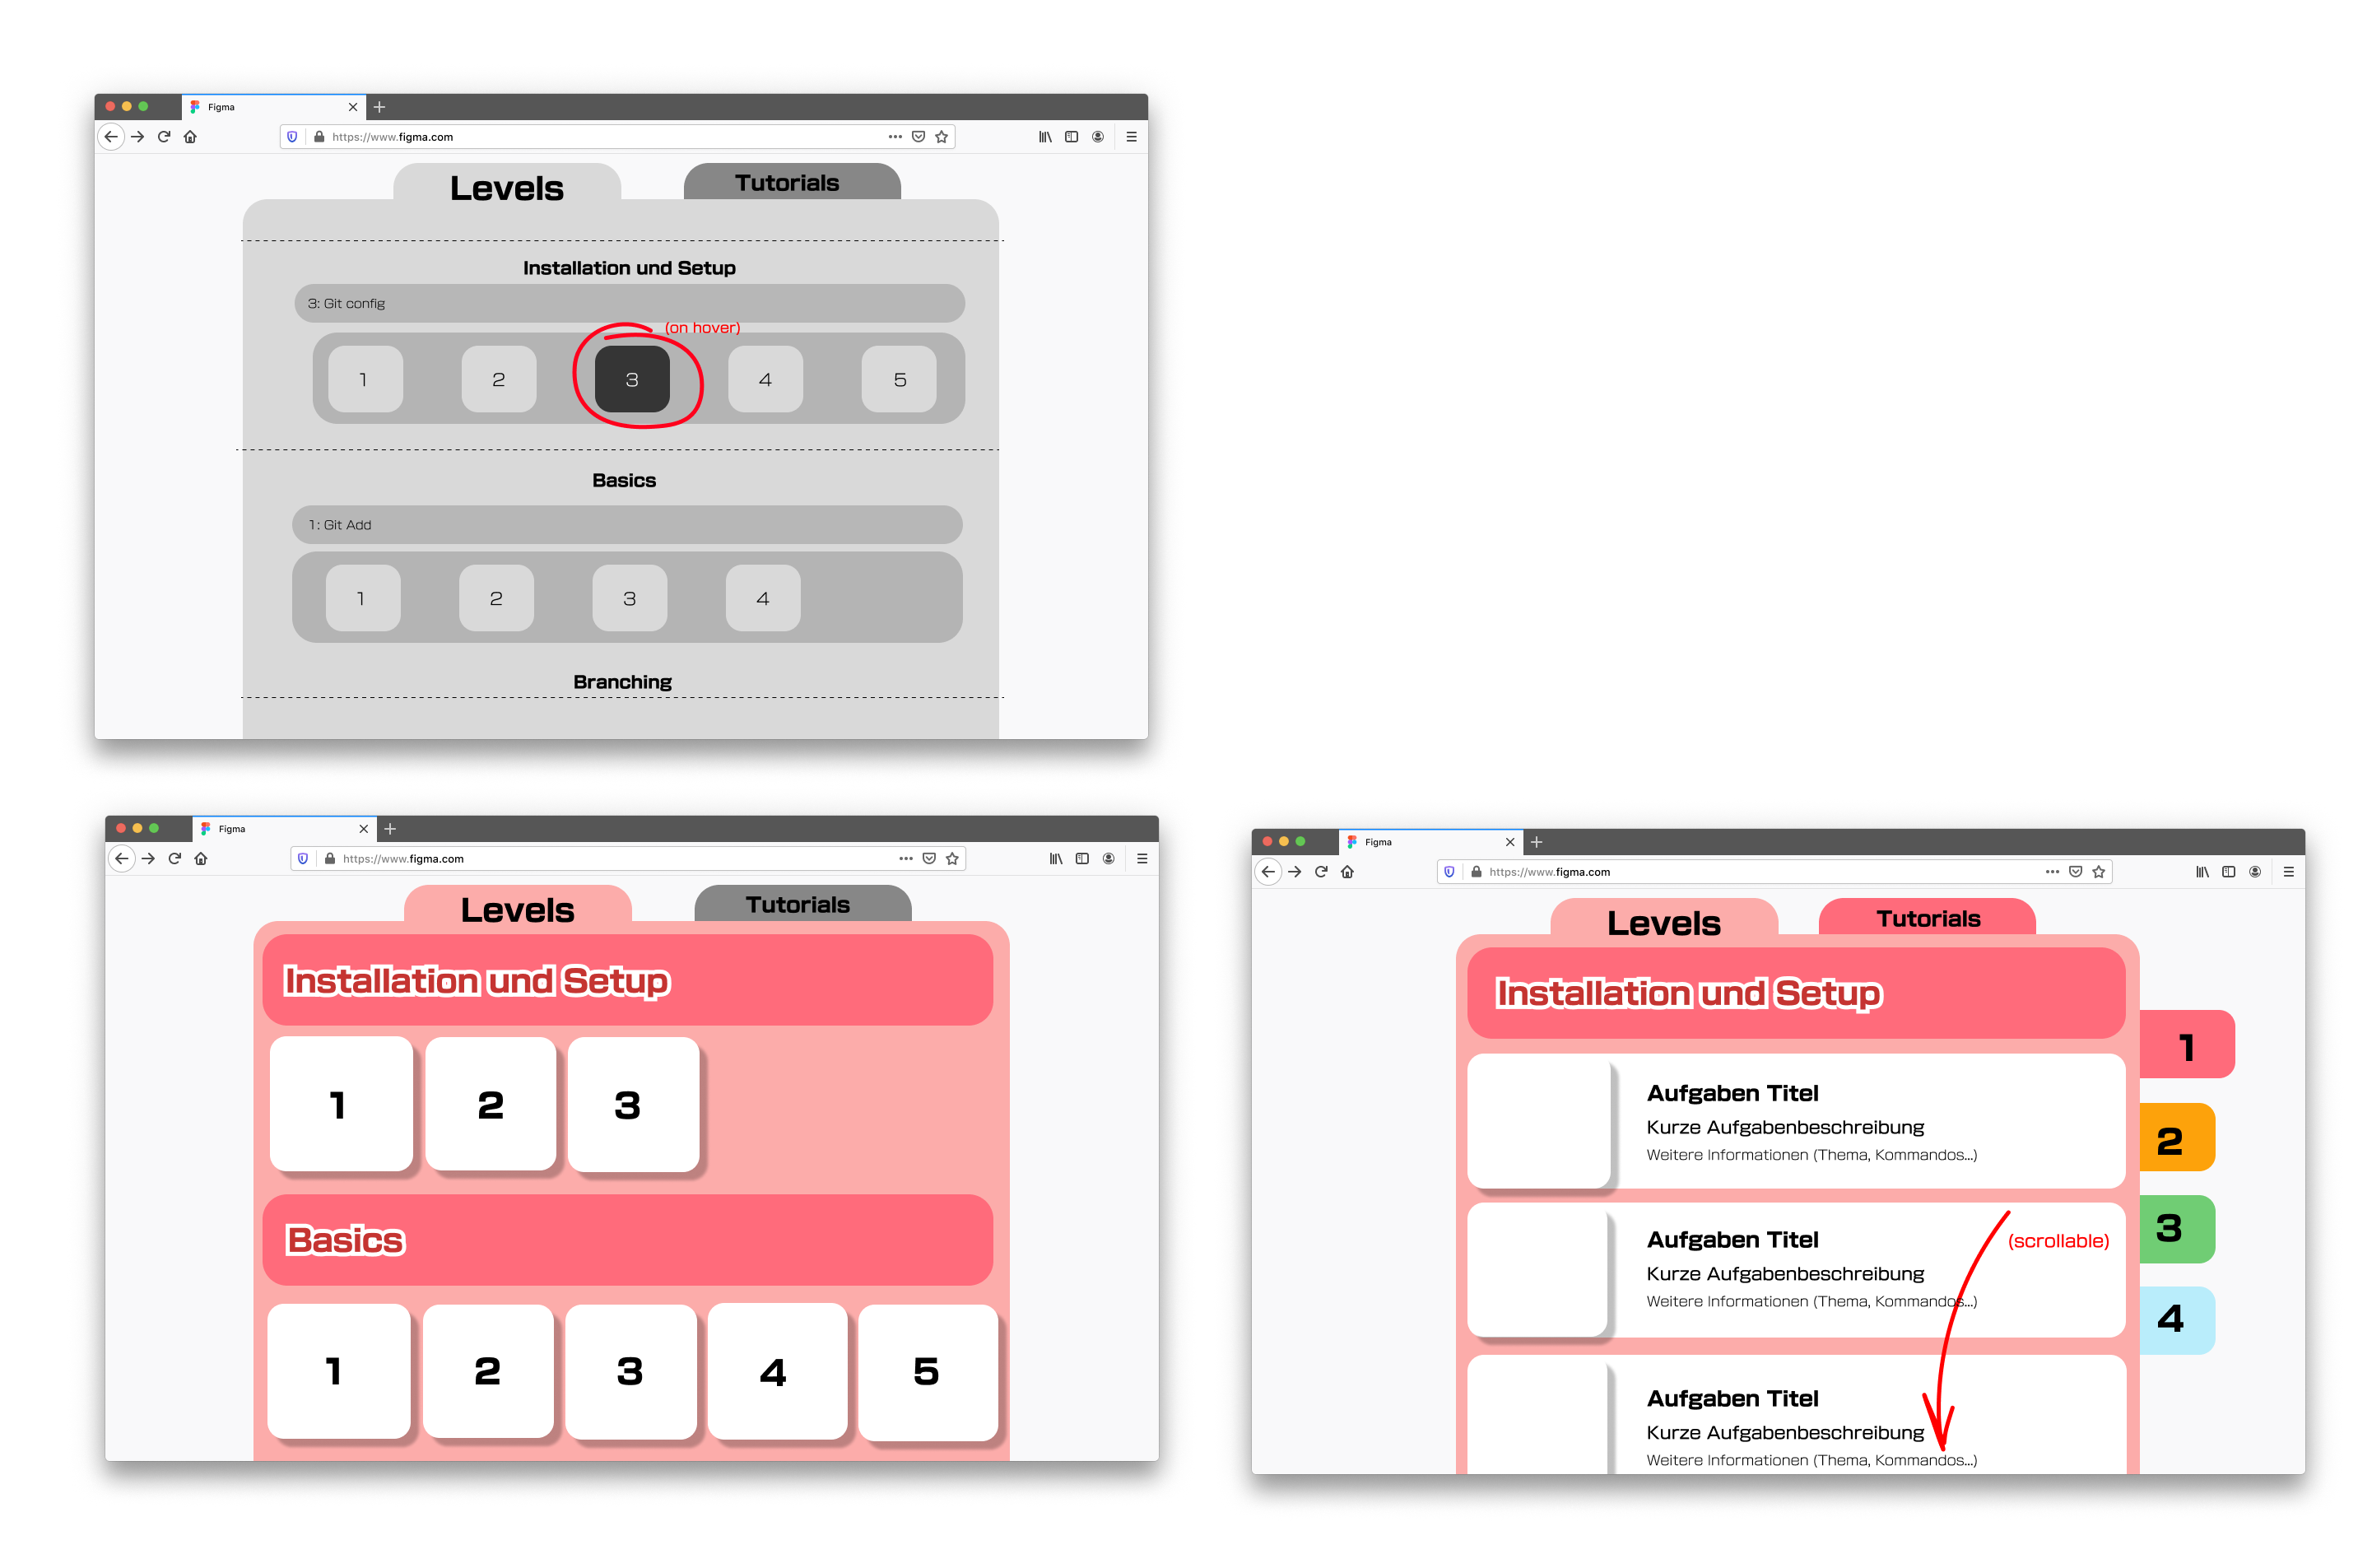
\includegraphics[width=\textwidth]{Wireframes_Level_V1}
    \caption{Wireframes zur Gestaltung der Levelauswahl}
\end{figure}

\begin{figure}[h!]
    \centering
    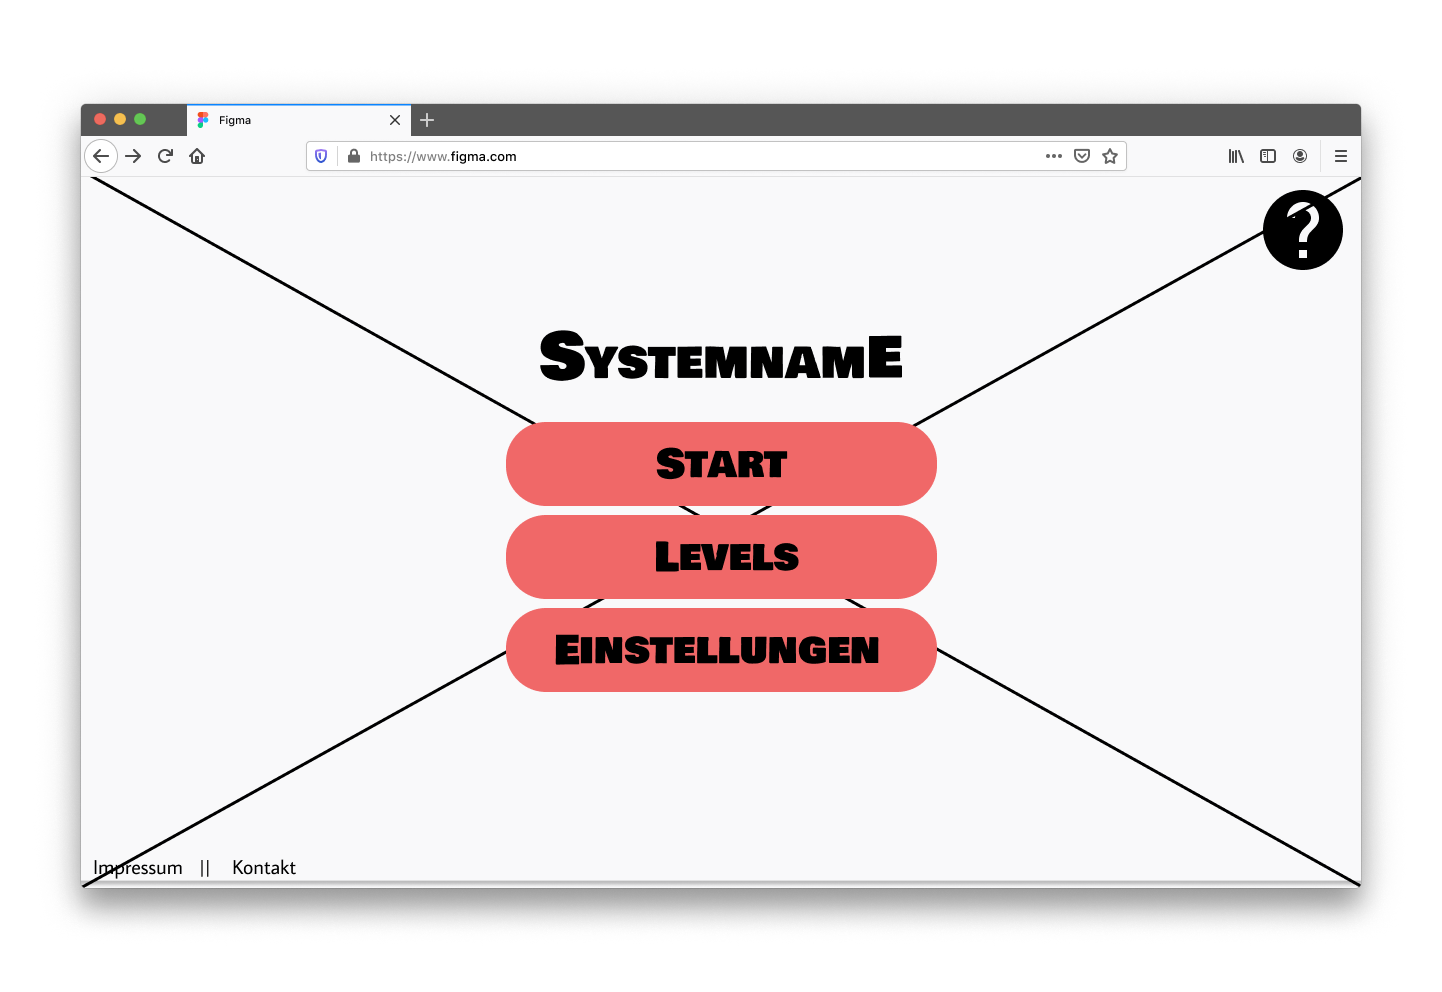
\includegraphics[width=\textwidth]{Wireframes_Homescreen_V1}
    \caption{Wireframes zur Gestaltung des Hauptmenüs}
\end{figure}

Die ersten Wireframes sollen die generelle Gestaltung der Menüs skizzieren.
Hierbei sollen alle Level in einer Art Bibliothek gesammelt sein. Die Levels sollen in einer beliebigen Reihenfolge gespielt werden können. Außerdem soll es noch einen weiteren Tab geben, um nur auf die Informationsinhalte zuzugreifen. Im Level selber befinden sich diese unter dem Informations-Button.
Durch eine separate Funktion hierbei soll sichergestellt werden, dass Studierende immer einfachen Zugriff auf alle Informationen haben und alle Kommandos mitsamt ihren Erklärungen an einem gesammelten Ort finden.

\begin{figure}[h!]
    \centering
    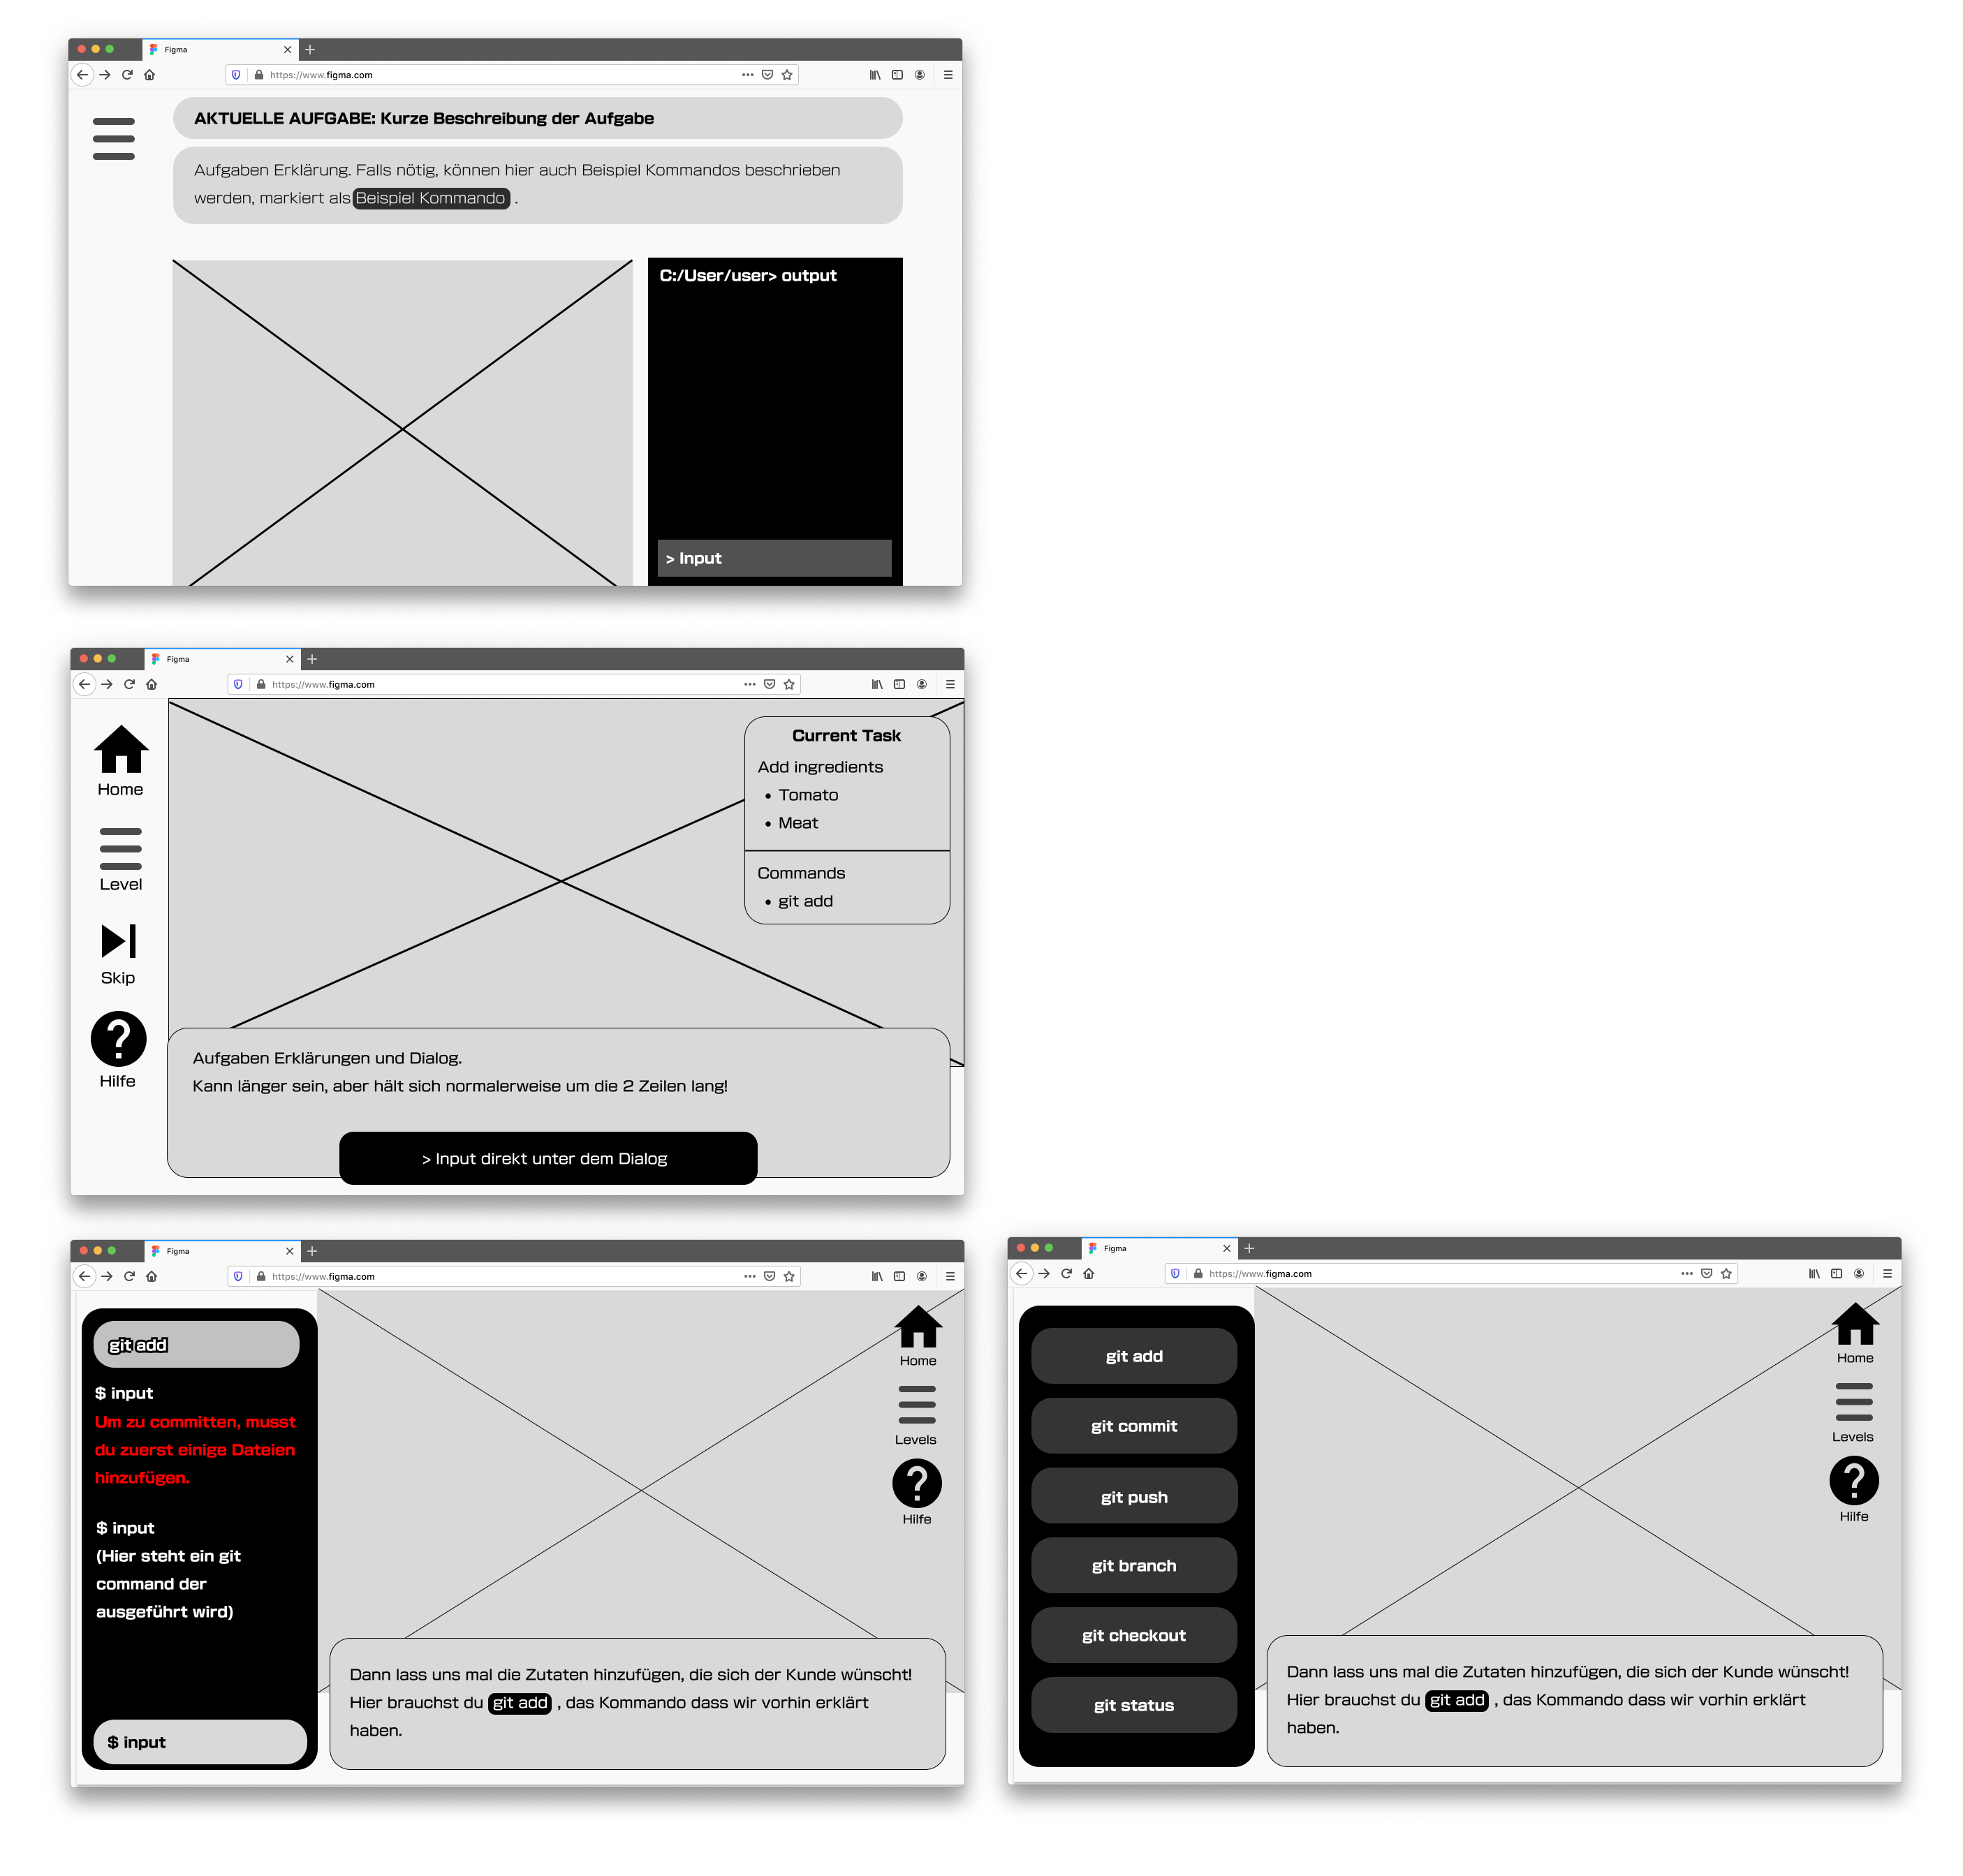
\includegraphics[width=\textwidth]{Wireframes_Aufgabe_V2}
    \caption{Wireframes zur Gestaltung des Spiele-Interface}
\end{figure}

Oben dargestellte Grafik soll die Planung des Leveldesigns verdeutlichen. Hierbei wurde unter anderem darauf geachtet, dass das User-Interface minimal gehalten wird, um unnötige Verwirrung zu vermeiden.
Über die Konsole sollen Eingaben getätigt werden, die in dem Bild mittig reflektiert werden. Zudem gibt es eine Menüleiste, in welcher der Nutzende gegebenenfalls ein Level überspringen kann, zurück ins Hauptmenü gelangt oder zusätzliche Erklärungen für das aktuelle Thema aufrufen kann.

Es wurden mehrere verschiedene Skizzen für das Interface erstellt. In der Umsetzung wurde letztendlich eine Kombination verwendet. Links sind die Menüpunkte zu finden, rechts an der Seite ist die Mock Konsole für Eingaben. Mittig in der finalen Version sind das Bild zum Szenario sowie die Dialogbox.